\chapter[Eddington Grey Atmosphere]{The Eddington Grey Atmosphere}

The following notes rely heavily on Mihalas, \emph{Stellar Atmospheres} and Shu, \emph{The Physics of Astrophysics}.

Let's start with the \emph{equation of transfer},
\begin{equation}\label{e.transfer}
\frac{1}{c}\partial_{t}I_{\nu} + \bvec{k}\cdot\grad I_{\nu} = \rho \frac{\varepsilon_{\nu}}{4\pi} - \rho\kappa_{\nu} I_{\nu} + \rho\kappa_{\nu}^{\mathrm{sca}}\phi_{\nu}
\end{equation}
for the specific intensity $I_{\nu}$, defined as the energy radiated per unit area per unit time per frequency per solid angle along a direction $\bvec{k}$. Here $\varepsilon_{\nu}$ is the energy spontaneously emitted per unit frequency per unit time per unit mass: the first term on the right hand side represents the energy added to the beam along a path $\dif s$.  The second term on the right hand side is the energy removed from the beam along a path $\dif s$ with $\kappa_{\nu} = \kappa_{\nu}^{\mathrm{abs}} + \kappa_{\nu}^{\mathrm{sca}}$ being the total opacity (absorption plus scattering). The last term is energy added to beam via scattering.  If the scattering is isotropic, then
\begin{equation}\label{e.isosca}
\phi_{\nu} = \frac{1}{4\pi}\int_{0}^{2\pi}\!\!\!\int_{0}^{\pi} I_{\nu}\,\dif\phi\,\sin\theta\,\dif\theta \equiv J_{\nu},
\end{equation}
where $J_{\nu}$ is the mean intensity: the scattering redistributes the energy over all angles.

\textbf{Moments of the intensity}
It is useful to define \emph{moments} of the specific intensity, which are just weighted angular averages.  For example, integrating $I_{\nu}$ over all angles and dividing by $4\pi$ gives
\begin{equation}\label{e.J}
J_{\nu} \equiv \frac{1}{4\pi}\int_{0}^{2\pi}\!\dif\phi\int_{0}^{\pi}\!\sin\theta\,\dif\theta\, I_{\mu} = \frac{1}{2}\int_{-1}^{1} \!\dif\mu \,I_{\nu}.
\end{equation}
Here $\mu = \cos\theta$. For the first moment, we can multiply $I_{\nu}$ by a unit vector $\bvec{k}$, and then dot that into the unit directional vector and integrate over all directions,
\begin{equation}\label{e.H}
H_{\nu} \equiv \frac{1}{4\pi}\int_{0}^{2\pi}\,\dif\phi\int_{0}^{\pi}\sin\theta\,\dif\theta\, I_{\mu}\,\bvec{k}\cdot\bvec{n} = \frac{1}{2}\int_{-1}^{1} \,\dif\mu \,\mu I_{\nu}.
\end{equation}
Finally, we can multiply $I_{\nu}$ by a tensor $\bvec{k}\bvec{k}$; contracting this along $\bvec{n}$ gives
\begin{equation}\label{e.K}
K_{\nu} \equiv \frac{1}{4\pi}\int_{0}^{2\pi}\,\dif\phi\int_{0}^{\pi}\sin\theta\,\dif\theta\, I_{\mu}\,(\bvec{k}\cdot\bvec{n})^{2} = \frac{1}{2}\int_{-1}^{1} \,\dif\mu \,\mu^{2} I_{\nu}.
\end{equation}
If we further integrate equations~(\ref{e.J})--(\ref{e.K}) over all frequencies, we will obtain expressions for the energy density, flux, and radiation pressure,
\begin{equation}\label{e.thermal}
u = \frac{4\pi}{c}J,\quad F = 4\pi H,\quad P = \frac{4\pi}{c}K.
\end{equation}

\textbf{Radiative equilibrium} The emissivity $\varepsilon_{\nu}$ and the opacity $\kappa_{\nu}$ describe how the radiation interacts with matter. If we imagine an irradiated atmosphere, then a condition of steady-state is that the gas not gain or lose energy to the radiation,
\begin{equation}\label{e.rad-equil}
\int_{0}^{\infty}\! \left(\frac{\varepsilon_{\nu}}{4\pi} - \kappa_{\nu}^{\mathrm{abs}} J_{\nu}\right)\,\dif\nu = 0.
\end{equation}
Now suppose that the level populations of the matter are in thermal equilibrium and can be described by a temperature $T$.  In that case, detailed balance must hold, so that
\begin{equation}\label{e.detail-balance}
\frac{\varepsilon_{\nu}}{4\pi\kappa_{\nu}^{\mathrm{abs}}} = B_{\nu}(T),
\end{equation}
where $B_{\nu}(T)$ is the Planck function. This defines \emph{local thermodynamic equilibrium (LTE)}. If the radiation field is, in addition, described by a Planck function \emph{at the same temperature} then we would have complete thermodynamic equilibrium.

\textbf{A plane-parallel atmosphere}
Now consider the time-independent problem ($\partial_{t}\to 0$) of a plane-parallel atmosphere. Define the \emph{optical depth} via the equation
\begin{equation}\label{e.optical-depth}
\tau_{\nu} = - \int _{z}^{\infty}\!\rho\kappa_{\nu}\,\dif r.
\end{equation}
Changing variables from $r$ to $\tau_{\nu}$, and defining $\mu = \bvec{k}\cdot\bvec{e}_{r}$ gives
\begin{equation}\label{e.planar}
\mu\frac{\partial I_{\nu}}{\partial\tau_{\nu}} = I_{\nu}-S_{\nu},
\end{equation}
where 
\begin{equation}\label{e.source}
S_{\nu} \equiv \frac{1}{\kappa_{\nu}}\left(\frac{\varepsilon_{\nu}}{4\pi} + \kappa_{\nu}^{\mathrm{sca}}J_{\nu}\right)
\end{equation}
is the \emph{source function}. In LTE, we can write $S_{\nu} = (1-A_{\nu})B_{\nu} + A_{\nu}J_{\nu}$, where $A_{\nu} \equiv \kappa_{\nu}^{\mathrm{sca}}/\kappa_{\nu}$ is the \emph{albedo}.

Now let's specialize to a grey atmosphere, i. e., one for which $\kappa_{\nu}^{\mathrm{abs}} = \kappa^{\mathrm{abs}}$ and $\kappa_{\nu}^{\mathrm{sca}} = \kappa^{\mathrm{sca}}$ are independent of frequency. Equation~(\ref{e.planar}) can then be integrated over all frequencies to become
\begin{equation}\label{e.J-grey}
\mu\frac{\partial I}{\partial\tau} = I-S.
\end{equation}
Integrating over all angles (note that we can pull the derivative wrt $\tau$ out of the integral) gives
\begin{equation}\label{e.H-grey}
\frac{\partial H}{\partial\tau} = J - S = 0.
\end{equation}
Why does the right-hand side vanish? Note that $S-J = (1-A)(B-J)$.  Clearly $S = J$ if $A = 1$ (a pure scattering atmosphere).  If $A \ne 1$, so that there is some absorption, then the condition of detailed balance, equation~(\ref{e.detail-balance}), implies that $\varepsilon_{\nu} = 4\pi\kappa^{\mathrm{abs}}B_{\nu}(T)$; inserting this into equation~(\ref{e.rad-equil}), factoring out the constant $\kappa^{\mathrm{abs}}$, and integrating over $\nu$ implies that $B - J = 0$, and hence $S = (1-A)B + AJ = J = B$. Note that $J = B$ does \emph{not} necessarily imply that $I_{\nu} = B_{\nu}$!

Finally, we can multiply equation~(\ref{e.J-grey}) by $\mu$ and integrate over angles to obtain
\begin{equation}\label{e.K-grey}
\frac{\partial K}{\partial\tau} = H,
\end{equation}
the integral over $\mu S$ vanishing because it is odd in $\mu$. Equation~(\ref{e.H-grey}) implies that $H$ is constant; hence we can integrate equation~(\ref{e.K-grey}) at once to obtain
\begin{equation}\label{e.KH}
K = H(\tau + \tau_{0}),
\end{equation}
where $\tau_{0}$ is a constant of integration.

\textbf{The Eddington Approximation}
Up to now, our derivation has been exact, to the extent that the approximation of a grey atmosphere in local thermodynamic equilibrium holds. To proceed, we still need a scheme to solve equation~(\ref{e.J-grey}). We have that $J = S$ in general, and as long as the atmosphere has some true absorption, $J = S = B$, but we still don't know $S(\tau)$. We could solve equation~(\ref{e.J-grey}) numerically via an iterative procedure. A more illuminating approach is to use the approximation made by Eddington. Observe that at great depth in the star, where not just radiative equilibrium but true thermal equilibrium holds, that the radiation field must obey the thermodynamic identity $P_{\mathrm{rad}} = u/3$. In terms of moments, this implies that $K = J/3$. Eddington noted that for an anisotropic radiation field, the departure from this identity is second-order; in other words, this approximation holds if the radiation is separately isotropic for outward-bound ($\mu > 0$) and inward-bound streams ($\mu < 0$).  Eddington therefore made the approximation that $K = J/3$ \emph{everywhere} in the atmosphere.

With this approximation, equation~(\ref{e.KH}) implies that $J = 3H(\tau + \tau_{0})$; further, since $J = S$, equation~(\ref{e.J-grey}) becomes
\begin{equation}
\mu\frac{\partial I}{\partial\tau} = I - 3H(\tau+\tau_{0}).
\end{equation}
This first-order differential equation (recall $H$ is constant) is then solvable,
\begin{eqnarray}
I(\mu,\tau=0) &=& \frac{1}{\mu}\int_{0}^{\infty}\!3H(\tau + \tau_{0}) e^{-\tau/\mu}\,\dif\tau,\nonumber\\
  &=& 3H(\mu + \tau_{0}).
\end{eqnarray}
Now at $\tau = 0$, all of the flux is outward-directed ($\mu >0$).  Let's multiply $I(\mu,\tau = 0)$ by $\mu$ and integrate to get $H$,
\begin{equation}
H = \frac{1}{2}\int_{0}^{1}\!\mu I(\mu,0)\,\dif\mu = \frac{1}{2}\int_{0}^{1}\!3H(\mu + \tau_{0})\,\mu\,\dif\mu = H\left(\frac{1}{2} + \frac{3}{4}\tau_{0}\right).
\end{equation}
This equation gives the constant, $\tau_{0} = 2/3$. Substituting $\tau_{0}$ into equation~(\ref{e.KH}), and rewriting $4\pi K = cP_{\mathrm{rad}}$, $4\pi H =  F = \sigma_{\mathrm{SB}}T_{\mathrm{eff}}^{4}$, gives at last the result,
\begin{equation}\label{e.Eddington}
T^{4}(\tau) = \frac{3}{4}T_{\mathrm{eff}}^{4}\left(\tau + \frac{2}{3}\right).
\end{equation}
This gives the temperature structure of the atmosphere.  To get the spectral distribution, go back to equation~(\ref{e.planar}) and (assuming the atmosphere has some absorption so that the matter and radiation can come into equilibrium) insert $S_{\nu} = B_{\nu}(T)$; solving for $I_{\nu}$ at $\tau = 0$ then gives
\begin{equation}\label{e.spectral}
I_{\nu}(\mu,\tau=0) = \frac{1}{\mu}\int_{0}^{\infty}\!B_{\nu}\left[T(\tau)\right] \, e^{-\tau/\mu}\,\dif\tau.
\end{equation}
A plot of the spectral distribution for the emergent flux is shown (\emph{open circles}) in Fig.~\ref{f.spectral}. For comparison, a plot of the Planck distribution (\emph{solid line}) is also shown. Both fluxes are normalized to the total flux.

\begin{figure}[htbp]
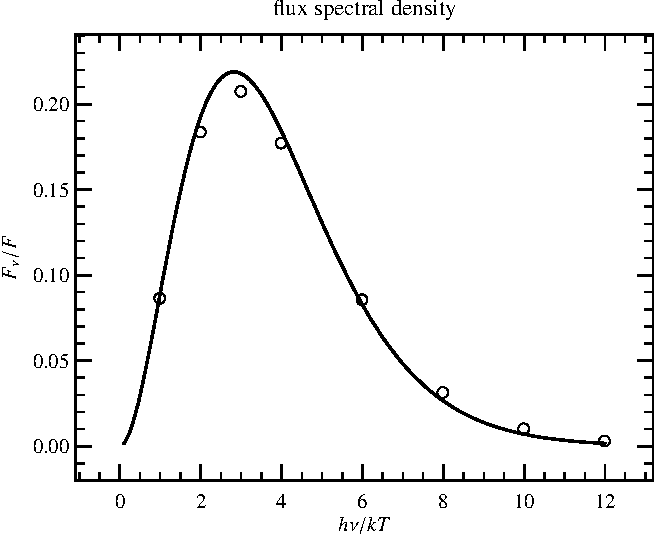
\includegraphics[width=4in]{plots_out/spectral_distribution}
\caption{\label{f.spectral} Spectral distribution from a grey atmosphere. The open circles are from Chandrasekhar, \emph{Radiative Transfer}; the solid line is the Planck distribution.}
\end{figure}
